\documentclass{article}
\usepackage[margin=1in,landscape]{geometry}
\newcommand{\overbar}[1]{\mkern 1.5mu\overline{\mkern-1.5mu#1\mkern-1.5mu}\mkern 1.5mu}
\pagenumbering{gobble}
\usepackage{tikz}

\begin{document}
\begin{center}
    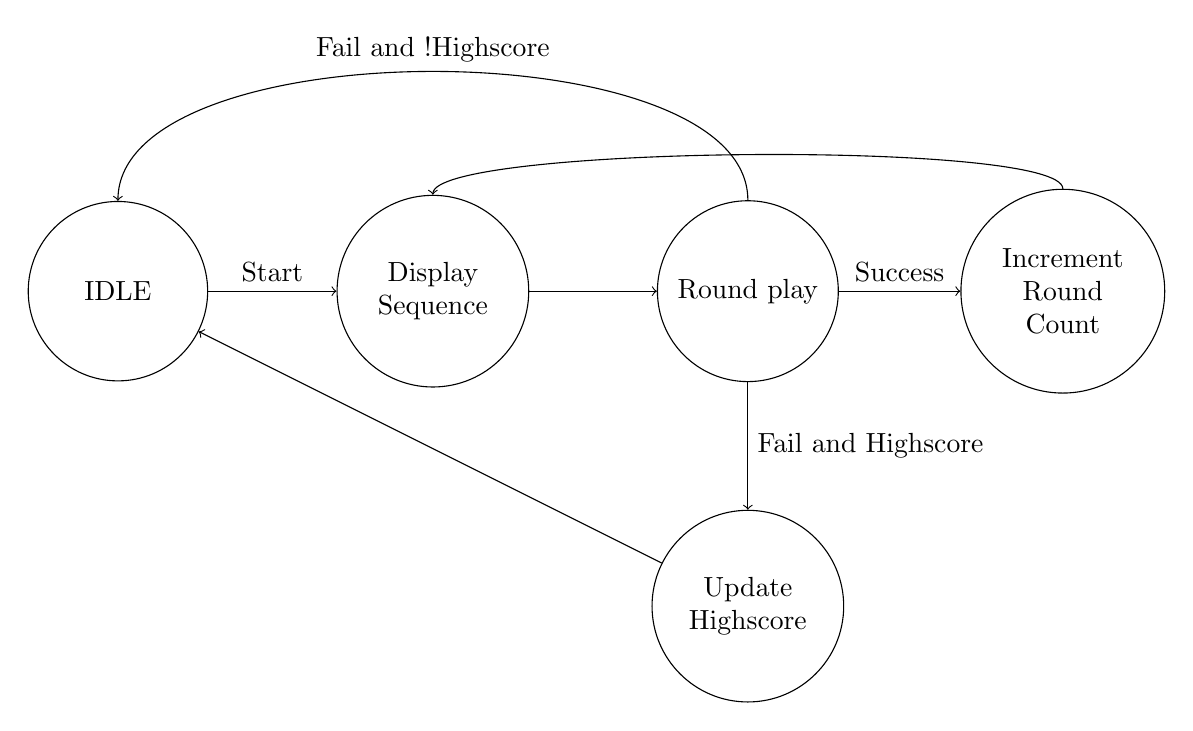
\begin{tikzpicture}[node distance={4cm},main/.style = {draw, circle,text width=2cm, text centered}]
        \node[main] (PowerOn) {IDLE};
        \node[main] (RoundStart) [right of = PowerOn]{Display Sequence};
        \node[main] (RoundPlay) [right of =RoundStart] {Round play};
        \node[main] (IncrementRound) [right of = RoundPlay] {Increment Round Count};
        \node[main] (UpdateHS) [below of = RoundPlay] {Update Highscore};
        \draw[->] (PowerOn) to node[above]{Start}(RoundStart);
        \draw[->] (RoundStart) to (RoundPlay);
        \draw[->] (RoundPlay) to node[above]{Success} (IncrementRound);
        \draw[->] (IncrementRound) to [in = 90, out = 90, looseness = 0.2]  (RoundStart);
        \draw[->] (RoundPlay) to [in = 90, out = 90, looseness = 0.7] node[above]{Fail and !Highscore} (PowerOn);
        \draw[->] (RoundPlay) to node[right]{Fail and Highscore} (UpdateHS);
        \draw[->] (UpdateHS) to (PowerOn);
    \end{tikzpicture}
\end{center}

\end{document}